\documentclass[hidelinks,a4paper,11pt]{article}
\usepackage[margin=2cm]{geometry}

\usepackage[titletoc,toc,title,page]{appendix}
\usepackage[nodayofweek]{datetime}
\usepackage{cite}
\usepackage{graphicx}
\longdate

\usepackage{hyperref}
\usepackage{fancyhdr}
\pagestyle{fancyplain}


\begin{document}

%%%%%%%%%%%%%%%%%%%%%%%%%%%%%%%%%%%%%%%%%%%%%%%%%%%%%%%%%%%%%%%%%%%%%%
%%%%%%%%%%%%%%%%%%%%%%%%%%%%%%%%%%%%%%%%%%%%%%%%%%%%%%%%%%%%%%%%%%%%%%
\section{Target animation}

%%%%%%%%%%%%%%%%%%%%%%%%%%%%%%%%%%%%%%%%%%%%%%%%%%%%%%%%%%%%%%%%%%%%%%
\subsection{Methodology}

This module represents the input to the dragonfly's retina. We needed to create an animation tool that allows the user to flexibly create a video of moving targets against a custom and potentially moving background. We started with the suggestion of creating a 3D animation where the dragonfly's view would change dynamically depending on the dragonfly's position and orientation but we decided that creating such an animation would be an overkill for our needs and too computationally expensive. Instead we settled with a 2D animation with coloured circles representing the targets against a moving or stationary 2D background. Our priorities were flexibility and simplicity. In the final output of the visual system, we would also want to be able to see the dragonfly chasing targets and we decided that, rather than create a whole new animation where the whole dragonfly is visible, it would make more sense to superimpose the dragonfly's visual focal point as a circle onto the original animation, so that the 'chasing' is represented as what point in its visual field the dragonfly is focusing on.  

The design of this module was approached from the user's perspective. The user would want to add targets, a background and get a final video. This could be done with 3 functions that would interact with an interface class. We named that class Animation. There were two types of targets: randomly moving ones and straight-line moving ones. For randomly moving ones, one could set a starting position and speed. In addition one should set a velocity vector for targets moving in straight line. The background is represented with the file location of an image and a speed with which we want it to move. Target and Background are both encapsulated in a class.

The next challenge was to turn this information into an animation. We decided to first create a sequence of images and turn them into an animation at the very end. This would allow us to easily superimpose the dragonfly focal point to the animation in the final stage of the system. We decided upon a Python module called Gizzet (CITATION) for image creation as it offers exactly what we needed – drawing circles, adding background images etc. in a user friendly way. We take the user's input to calculate position of each target and of background at each frame. Using that calculation we know where to draw circles and background picture, afterwards we save the created image.

The generated sequence of images is than combined into a video using OpenCV (CITATION) and exported under a selected filename. Additionally, the module outputs the series of images in matrix format of pixel values to be passed to the ESTMD module.

In addition to the above functionality of target animation module, we needed to somehow pass data of target positions to the final module – the action selection – in order to assist with the reward-modulated learning and to superimpose the position of the dragonfly's focal point onto the animation, which is determined by this final module. To satisfy this need we added functions that calculate positions of targets at a certain time during the animation.

Example of frame in produced video can be seen on the picture  ~\ref{target_animation_example}.

\begin{figure}[hb]
\centering
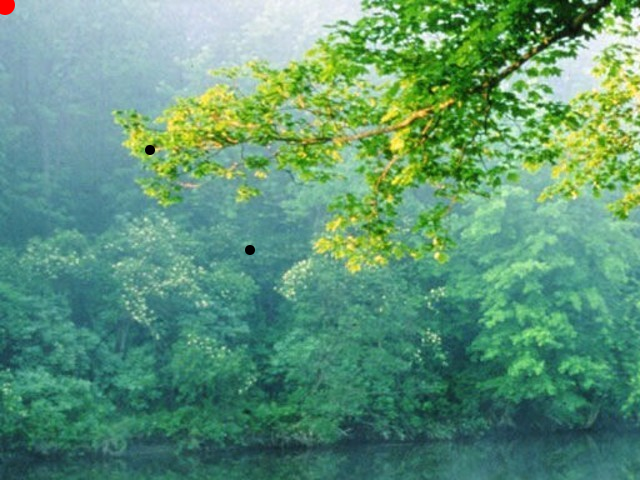
\includegraphics[scale = 0.3]{example}
\caption{Simple example of action selection output. The red dot represents the dragonfly focal point and the black dot represents the target.}
\label{target_animation_example}
\end{figure}

\newpage

%%%%%%%%%%%%%%%%%%%%%%%%%%%%%%%%%%%%%%%%%%%%%%%%%%%%%%%%%%%%%%%%%%%%%%
\subsection{Final product}

Here is the breakdown of the final product down in classes.
\\
\\
Animation:
Interface that the user interacts with.
\\
Methods:
\begin{itemize}
\item add target
\item add background
\item add dragonfly
\item get target positions
\end{itemize}

Other classes used were Target, Dragonfly, Backround and AnimationWindow. I can bullshit about any of them unlimitedly.



%%%%%%%%%%%%%%%%%%%%%%%%%%%%%%%%%%%%%%%%%%%%%%%%%%%%%%%%%%%%%%%%%%%%%%
%%%%%%%%%%%%%%%%%%%%%%%%%%%%%%%%%%%%%%%%%%%%%%%%%%%%%%%%%%%%%%%%%%%%%%
\end{document}

